\begin{figure}
	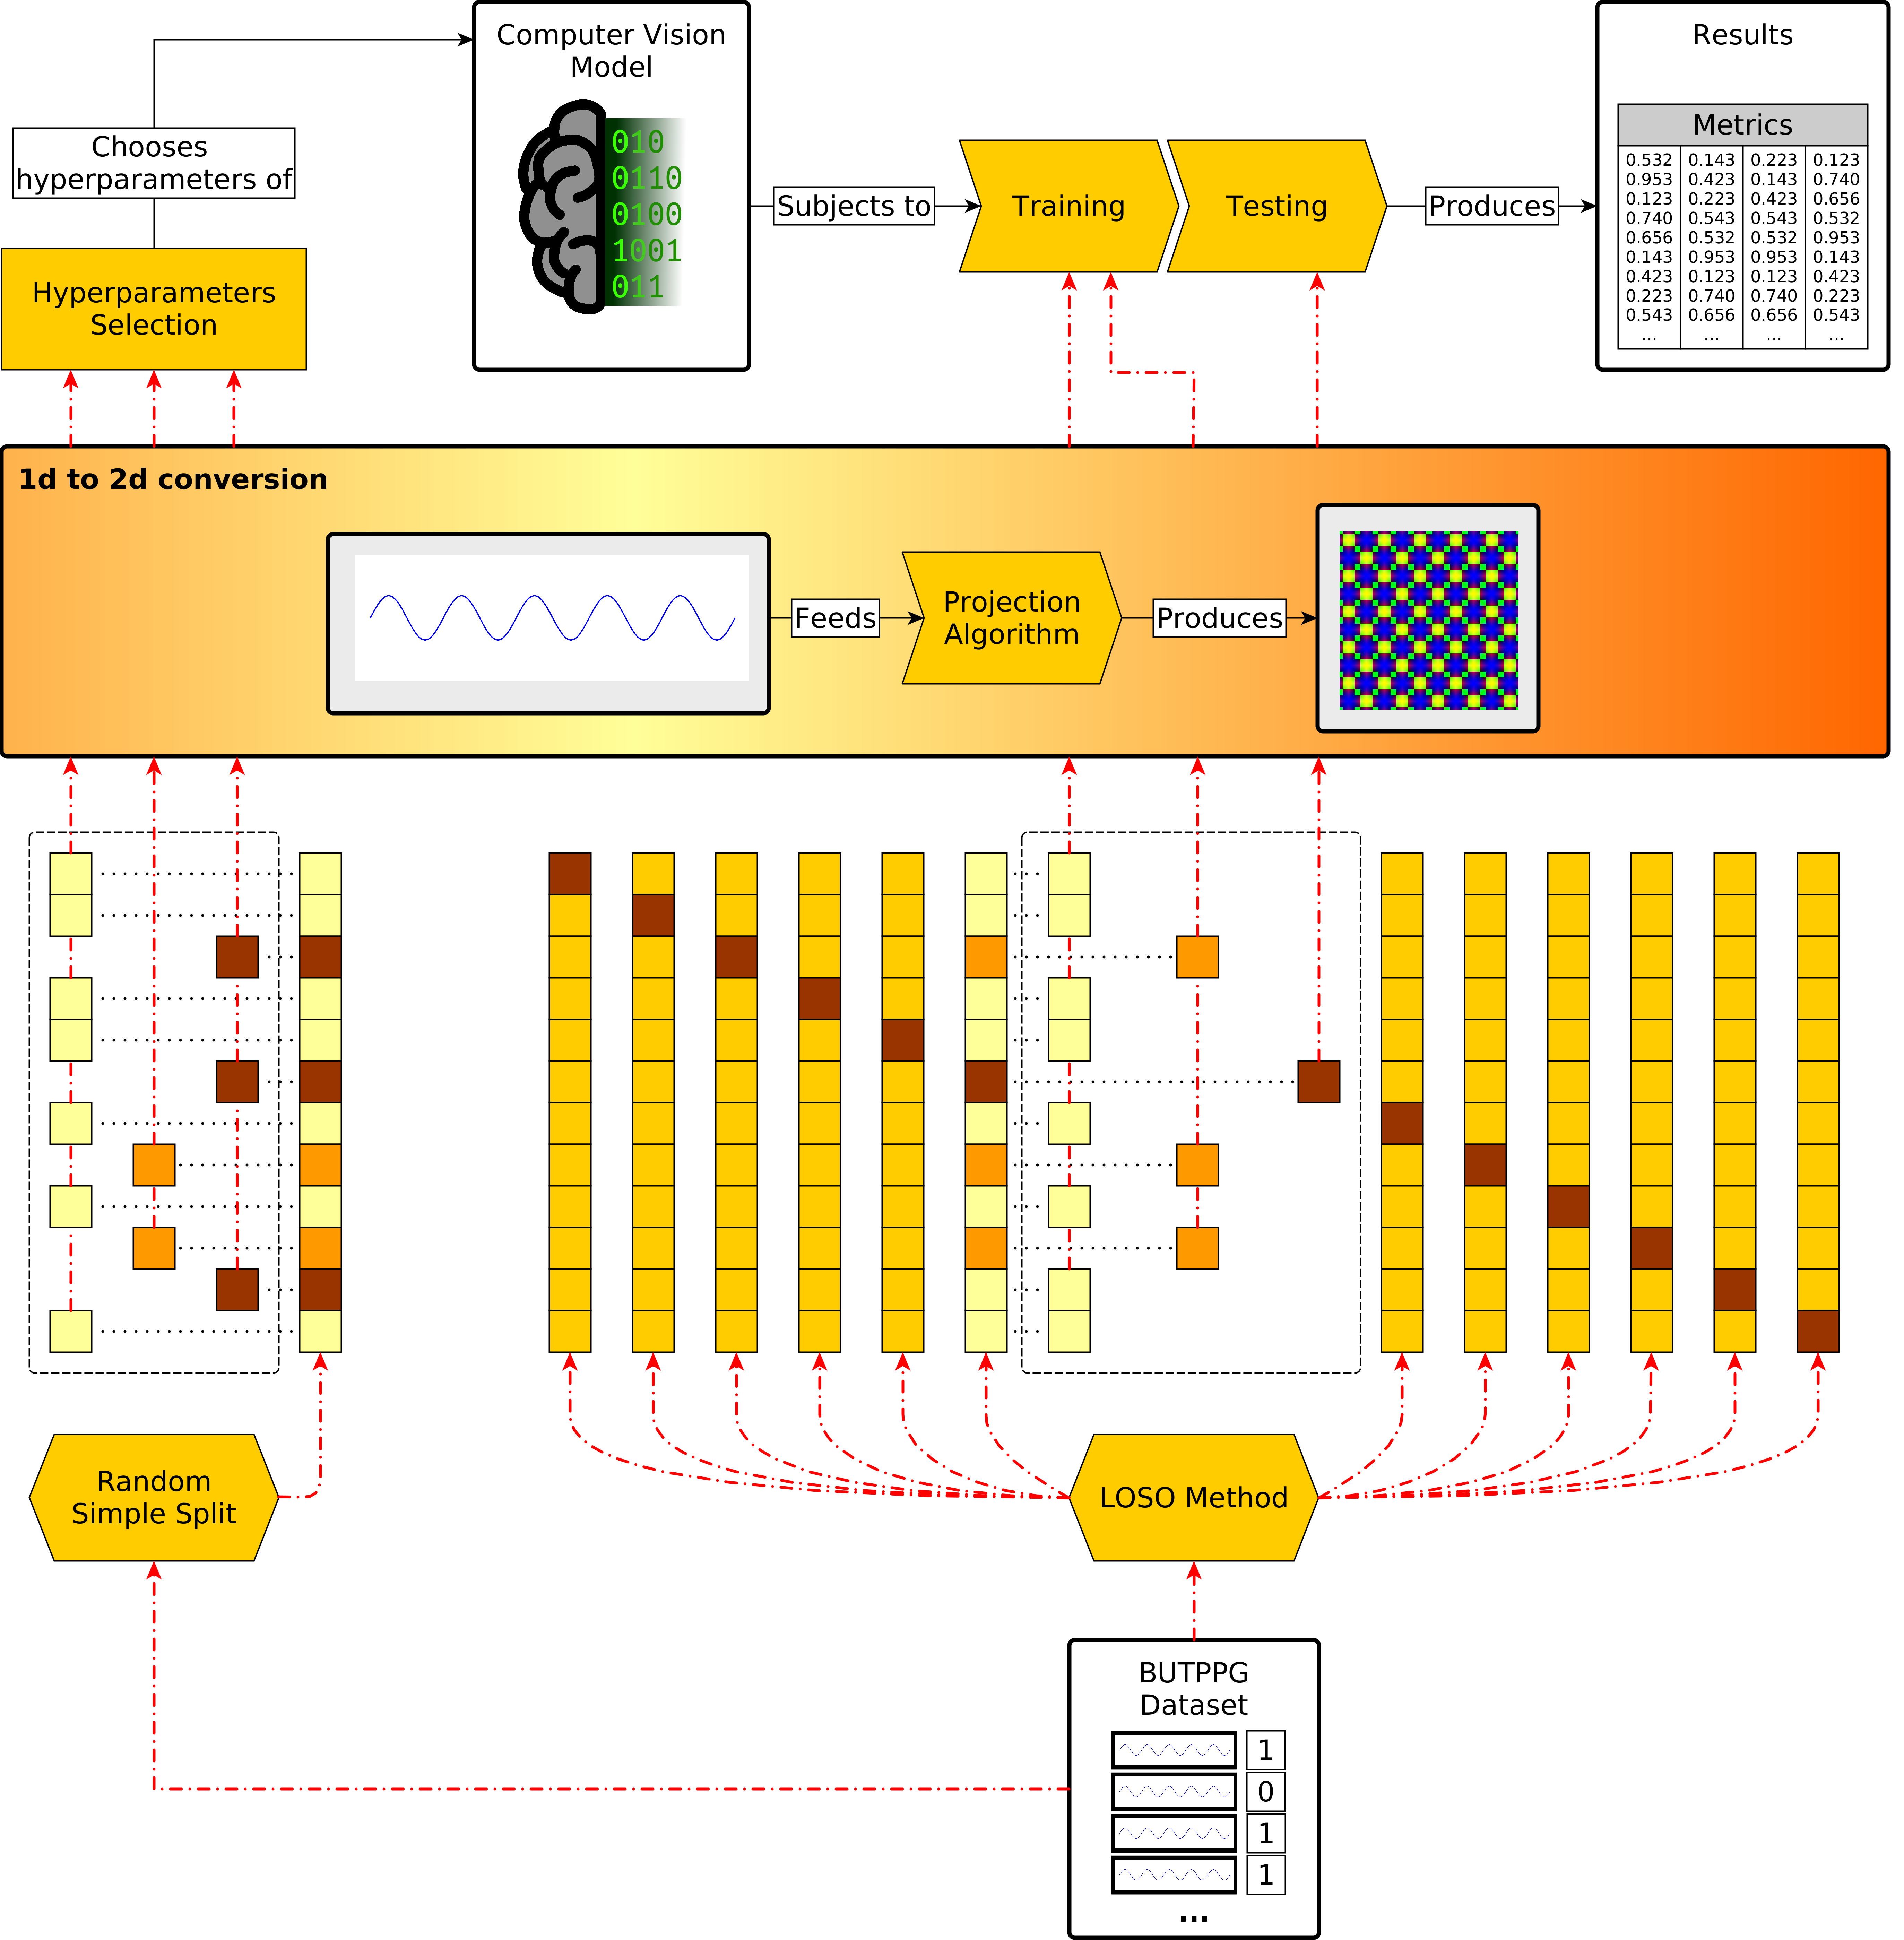
\includegraphics[width=\textwidth]{img/framework.png}
	\caption[The framework of the experiment.]{The framework of the experiment. Red dotted arrows indicates data flow that sources from the \acrlong{BUTPPG} dataset, while the full black lines, labeled with an verb, represent a relationship ``A do B'', where the arrow starts on A and end on B. Notice that the figure presents the training-testing cycle for only one of the twelve folds.}
	\label{fig:framework}
\end{figure}
